
\section{Appendix}
\label{sec:appendix}

\subsection{Additional Graphs for Performance of Brute Force versus k-d Trees}

\begin{figure}[H]
\centering
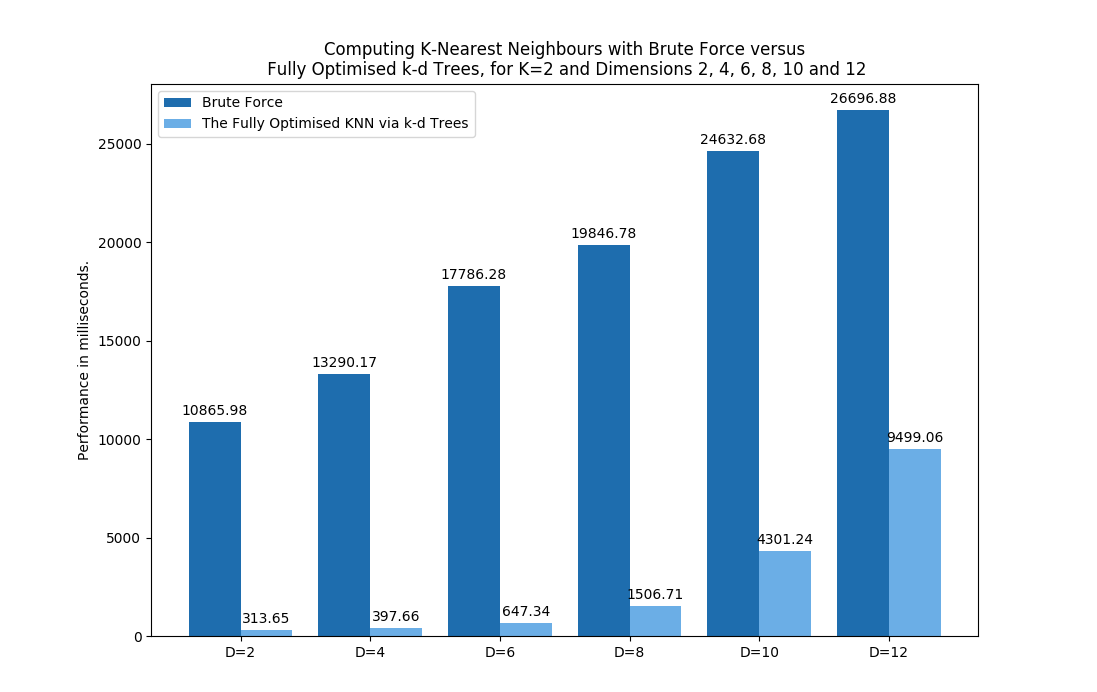
\includegraphics[width=1\textwidth]{pics/plot-figs/new-brute-k2.png}
\caption{Performance comparison of k-d tree versus brute force, with a static K=2 on datasets of sizes 1048576.}
\label{fig:b1}
\end{figure}


\begin{figure}[H]
\centering
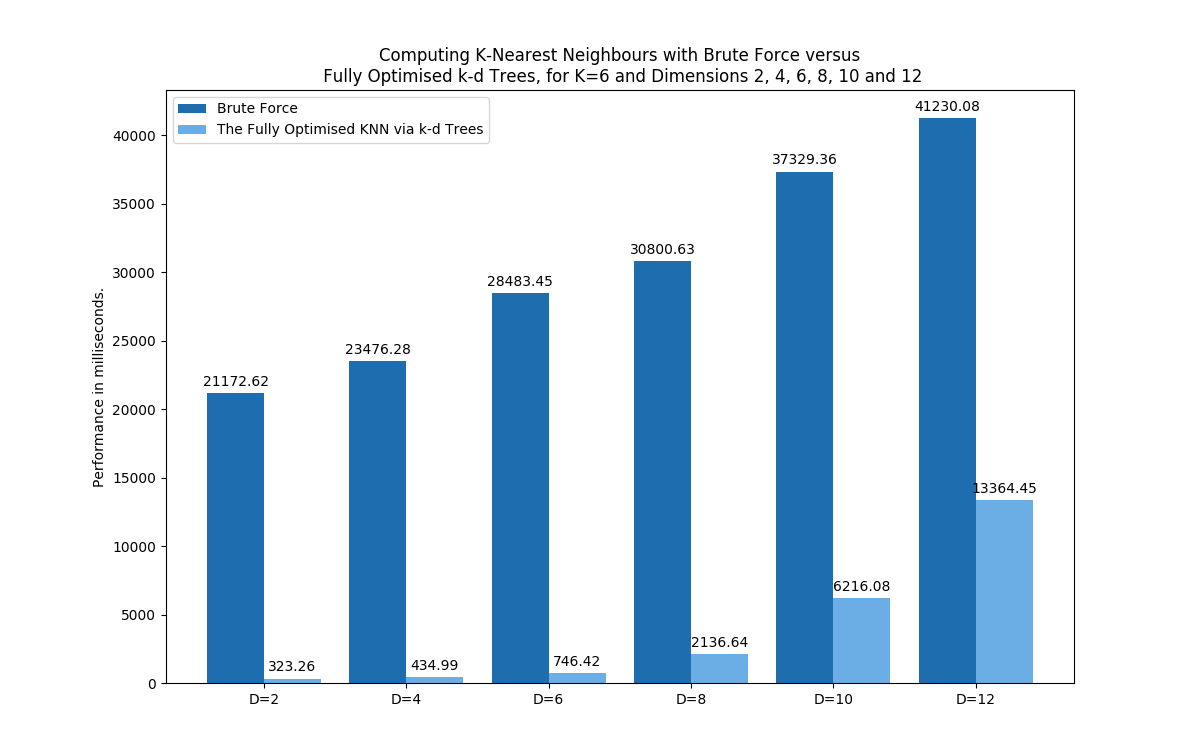
\includegraphics[width=1\textwidth]{pics/plot-figs/new-brute-k6.png}
\caption{Performance comparison of k-d tree versus brute force, with a static K=6 on datasets of sizes 1048576.}
\label{fig:b2}
\end{figure}


\begin{figure}[H]
\centering
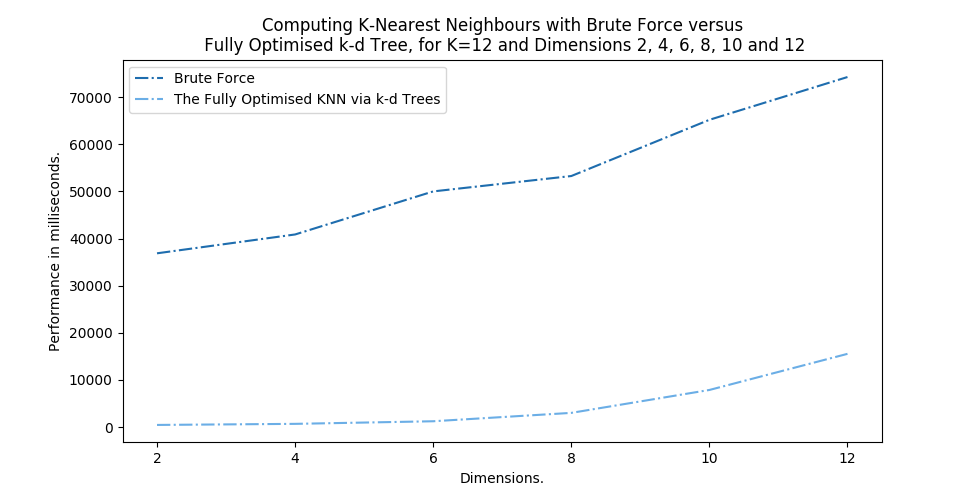
\includegraphics[width=1\textwidth]{pics/plot-figs/new-brute-k12-lines.png}
\caption{Performance comparison of k-d tree versus brute force, with a static K=12 on datasets of sizes 1048576.}
\label{fig:b4}
\end{figure}



\begin{figure}[H]
\centering
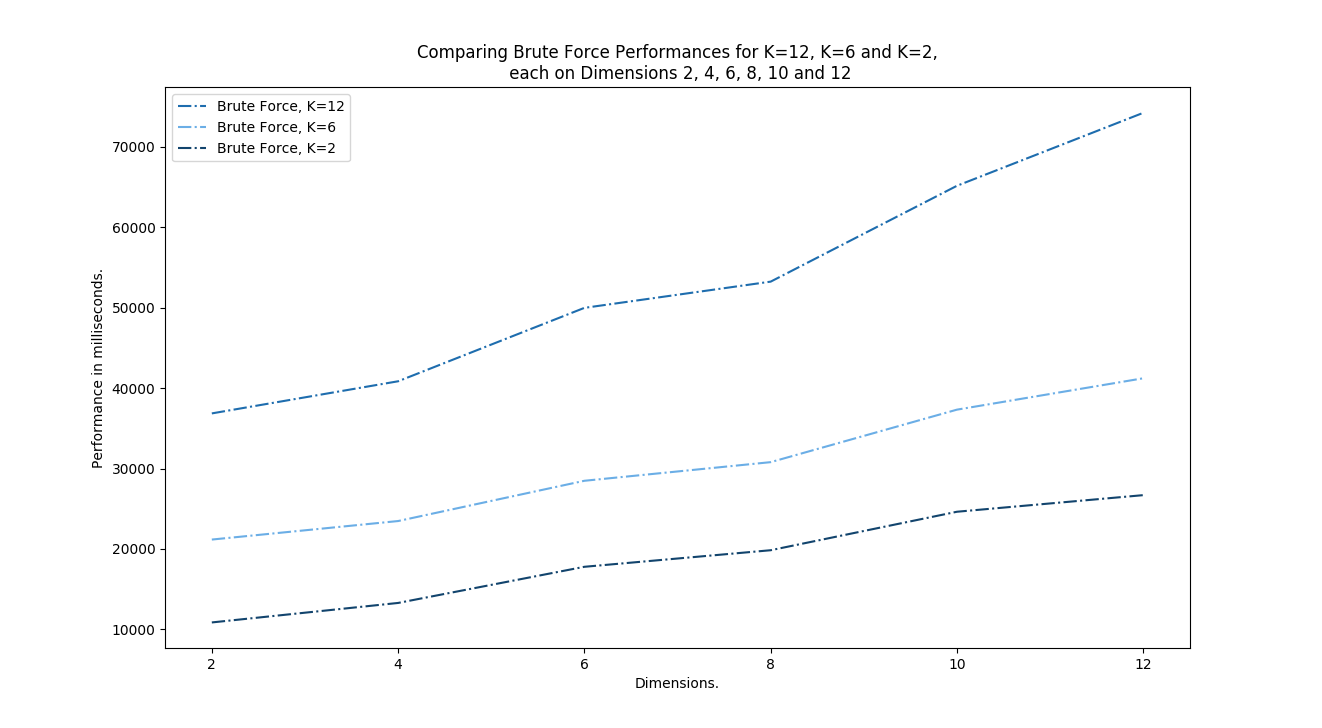
\includegraphics[width=1\textwidth]{pics/plot-figs/brute-k2k6k12.png}
\caption{Performance comparison of brute force, with K=12, K=6 and K=2, on datasets of sizes 1048576.}
\label{fig:b6}
\end{figure}


\begin{figure}[H]
\centering
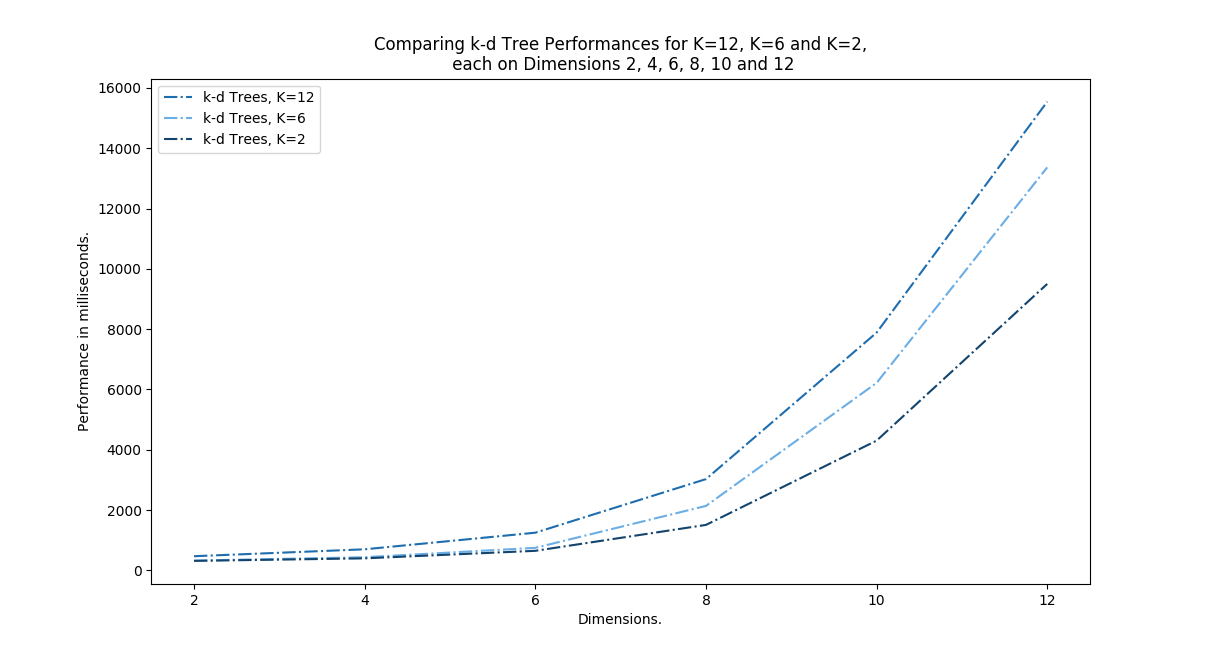
\includegraphics[width=1\textwidth]{pics/plot-figs/kdtree-k2k6k12.png}
\caption{Performance comparison of k-d tree, with K=12, K=6 and K=2, on datasets of sizes 1048576.}
\label{fig:b7}
\end{figure}


